\documentclass[journal]{IEEEtran}

\usepackage{cite}
\usepackage{textcomp}
\def\BibTeX{{\rm B\kern-.05em{\sc i\kern-.025em b}\kern-.08em
     T\kern-.1667em\lower.7ex\hbox{E}\kern-.125emX}}
\providecommand{\keywords}[1]{\textbf{\textit{Keywords:}} #1}
\usepackage{graphicx}
\usepackage{booktabs}
\usepackage[utf8]{inputenc}
\usepackage[english, activeacute]{babel}
\usepackage{float}
\usepackage{amssymb}
\usepackage{amsmath}
\usepackage{mathrsfs}
\usepackage{amsbsy}
\usepackage{hyperref}
\usepackage{algorithm}
\usepackage{algpseudocode}
\usepackage{array}
\usepackage[table]{xcolor}
\usepackage{colortbl}
\usepackage{mathtools}
\usepackage{tikz}
\usetikzlibrary{positioning, arrows.meta, shapes.geometric, calc, decorations.pathmorphing, patterns, fit, plotmarks}
\usepackage{verbatim}
\pagestyle{plain}
\usepackage[switch]{lineno}
\hyphenation{op-tical net-works semi-conduc-tor}

\begin{document}
\raggedbottom

\title{Priority-Aware Task Offloading and 3D Trajectory Optimization in NOMA-Enabled Multi-UAV MEC-IoT Networks Using MAPPO}

\author{Nayanjit~Talukdar, Kushagra~Gupta, Krishna~Sikheriya, Aditya~Pankaj~Sharma,
    Nabajyoti~Mazumdar,~\IEEEmembership{~Senior Member, IEEE}
    \thanks{\emph{(Corresponding author: Nabajyoti Mazumdar.)}}
    \thanks{K.~Gupta (student ID: IIT2023133), K.~Sikheriya (student ID: IIT2023139), and A.~P.~Sharma (student ID: IIT2023162) are B.Tech.\ students. N.~Talukdar is a Ph.D.\ Scholar. All four are with the Department of Information Technology, Indian Institute of Information Technology, Allahabad, India. N.~Mazumdar is an Assistant Professor with the same department. (e-mail: \texttt{nabajyoti@iiita.ac.in}).}
}

\maketitle

%% ============================================================
%%  ABSTRACT
%% ============================================================
\begin{abstract}
Integrating unmanned aerial vehicles (UAVs) with mobile edge computing (MEC) establishes an agile paradigm for provisioning compute capabilities to energy-constrained Internet of Things (IoT) nodes in dynamic, infrastructure-deficient environments. Nevertheless, prevailing computation offloading architectures conventionally treat workloads uniformly, failing to accommodate the heterogeneous urgency, delay tolerances, and operational criticality inherent to real-world sensory deployments. Furthermore, simultaneously steering multi-UAV 3D trajectories, managing non-orthogonal multiple access (NOMA) uplink interference, and scheduling priority-differentiated tasks under strict aerial propulsion limits constitutes a high-dimensional, tightly coupled mixed-integer non-convex challenge. To address these bottlenecks, this paper proposes the \textit{Priority-Aware Multi-UAV Joint Optimization (PA-MUJO)} framework. We formulate the joint problem as a stochastic mixed-integer nonlinear program (MINLP) and devise a multi-agent proximal policy optimization (MAPPO) scheme operating under the centralized training with decentralized execution (CTDE) architecture. A composite priority characterization is established to dynamically weigh task urgency against application criticality, enabling the aerial fleet to preferentially schedule and compute high-priority requests. To mitigate reinforcement learning action complexity, NOMA uplink transmit powers are determined analytically via bisection search, decoupling physical transmission control from actor policy gradient updates. Extensive simulations demonstrate that PA-MUJO considerably curtails priority-penalized execution latency and economizes UAV propulsion energy relative to state-of-the-art benchmarks, exhibiting resilient multi-agent spatial coordination.
\end{abstract}

\begin{IEEEkeywords}
Unmanned aerial vehicles (UAVs), mobile edge computing (MEC), Internet of Things (IoT), multi-agent reinforcement learning (MARL), non-orthogonal multiple access (NOMA), priority-aware offloading, 3D trajectory design.
\end{IEEEkeywords}

%% ============================================================
%%  I. INTRODUCTION
%% ============================================================
\section{Introduction}

\IEEEPARstart{T}{he} proliferation of the Internet of Things (IoT) has accelerated the deployment of autonomous sensory and embedded devices across smart transportation, industrial telemetry, environmental surveillance, and emergency response~\cite{liu2025integrated, mao2017mec}. In these applications, ground devices (GDs) continuously collect observational telemetry and produce computational workloads requiring near-instantaneous execution. However, typical GDs operate under stringent hardware limits, including miniature battery capacities and restricted processor clock frequencies. Executing data-intensive algorithms on-device rapidly depletes local energy reserves and induces severe processing latency~\cite{zhan2026joint, barman2025joint}. Mobile edge computing (MEC) mitigates this physical constraint by deploying computing servers at the network edge, enabling resource-limited terminals to offload demanding workloads via wireless channels~\cite{mao2017mec, 11020655}.

Despite the benefits of MEC, conventional terrestrial edge architectures rely on stationary base stations whose fixed geographic footprint renders them vulnerable to physical obstructions, severe propagation shadowing, and exorbitant deployment overhead in remote or devastated areas~\cite{li2026tnse, zeng2019accessing}. To circumvent these physical bottlenecks, unmanned aerial servers carrying onboard edge computing payloads have emerged as an agile, on-demand paradigm~\cite{kang2023cooperative, tariq2024toward}. Leveraging high spatial maneuverability and line-of-sight (LoS) air-to-ground (A2G) propagation, a cooperative fleet of rotary-wing UAVs can dynamically relocate across three-dimensional (3D) airspace, provisioning elastic edge compute capacity and adaptive coverage directly above dispersed ground terminals~\cite{11500527, li2026tnse}.

Nevertheless, orchestrating cooperative multi-UAV MEC networks presents three critical unresolved challenges:
\begin{enumerate}
    \item \textit{Workload Urgency Disparities and Priority Inversion:} Existing offloading literature predominantly presumes homogeneous workload characteristics, treating incoming tasks uniformly through first-come-first-served scheduling~\cite{yang2026drl, tariq2024toward, barman2025joint}. Real-world IoT deployments, however, exhibit extreme variations in operational urgency; emergency alarms and vehicular collision avoidance tolerate only millisecond-level delays, whereas periodic telemetry tolerates relaxed deadlines~\cite{hu2020priority, sun2023priority}. Indiscriminate resource allocation induces ``priority inversion,'' where delay-tolerant background traffic monopolizes scarce aerial computing and spectral resources, resulting in fatal deadline expirations for mission-critical tasks~\cite{sun2023priority, peng2024priority}.
    \item \textit{3D Flight Kinodynamics and Non-Linear Aerodynamic Expenditure:} Most existing trajectory schemes restrict aerial navigation to fixed two-dimensional (2D) planes~\cite{tariq2024toward, sun2023priority}. While vertical elevation adjustments dynamically regulate LoS channel probabilities and overcome terrestrial shadowing~\cite{li2026tnse}, rotary-wing aerodynamic propulsion power varies non-linearly with airspeed, dominating onboard battery depletion by orders of magnitude over computing circuitry~\cite{8937764, li2026tnse}. Balancing dynamic propagation enhancements against severe propulsion energy drains in 3D airspace under multi-UAV collision constraints remains an open challenge.
    \item \textit{Action Space Dimensionality in NOMA Uplink Power Control:} Uplink power-domain non-orthogonal multiple access (NOMA) enables multiple GDs to simultaneously offload over identical spectral bands via successive interference cancellation (SIC)~\cite{11020655, qin2024drl, 10697399}. However, directly parameterizing continuous device transmit powers inside reinforcement learning actor action spaces causes severe policy gradient variance and dimensional explosion, destabilizing multi-agent convergence.
\end{enumerate}

To overcome these hurdles, this paper introduces the \textit{Priority-Aware Multi-UAV Joint Optimization (PA-MUJO)} framework. We formulate the joint problem of 3D aerial navigation, priority-differentiated task offloading, and NOMA uplink transmission as a stochastic mixed-integer non-linear program (MINLP) to minimize the priority-weighted aggregate latency while regulating UAV propulsion and computing energy expenditure. To resolve this combinatorial formulation, we develop a multi-agent proximal policy optimization (MAPPO) algorithm under the centralized training with decentralized execution (CTDE) architecture~\cite{kang2023cooperative, yu2022mappo}. Crucially, we establish an analytical-RL hybrid decoupling: decentralized UAV actors govern macro-level spatial movement and scheduling associations, while optimal NOMA transmit powers are determined analytically via convex bisection, guaranteeing quality-of-service (QoS) rates while stabilizing policy training.

The principal contributions of this work are summarized as follows:
\begin{itemize}
    \item \textbf{Comprehensive Stochastic MINLP Formulation:} We establish an end-to-end multi-UAV MEC-IoT framework integrating Gauss-Markov ground device mobility, probabilistic elevation-dependent A2G channels, NOMA uplink interference, UAV edge queueing dynamics, and non-linear rotary-wing aerodynamics under strict battery and inter-UAV collision bounds.
    \item \textbf{Composite Urgency-Criticality Priority Model:} We design a composite priority metric fusing real-time deadline margins with semantic application criticality. Penalizing delay proportionally to priority directs the aerial fleet to preferentially schedule and execute time-critical workloads, fundamentally eliminating priority inversion.
    \item \textbf{Analytical Decoupling of NOMA Power Allocation:} We derive a recursive closed-form bisection algorithm for uplink NOMA transmission powers, completely eliminating continuous power control from the RL action space and drastically accelerating policy convergence.
    \item \textbf{CTDE-Based MAPPO Fleet Coordination:} We implement a MAPPO cooperative optimization scheme with Generalized Advantage Estimation (GAE) and clipped surrogate objectives, validated via comprehensive simulations demonstrating superior priority latency reduction, energy conservation, and collision-free spatial coordination over state-of-the-art baselines.
\end{itemize}

The structural layout of this article proceeds as follows: Section~\ref{sec_II} examines related scholarly works. Section~\ref{section_III} details the system architecture and mathematical formulation. Section~\ref{section_IV} establishes the cooperative PA-MUJO algorithm and bisection power allocation. Section~\ref{section_V} analyzes numerical performance results, and Section~\ref{con} summarizes conclusions and future trajectories.


%% ============================================================
%%  II. RELATED WORK
%% ============================================================
\section{Related Work}
\label{sec_II}

\subsection{Computation Offloading in UAV-Assisted MEC Systems}

Deploying unmanned aerial vehicles (UAVs) equipped with mobile edge computing (MEC) servers has emerged as an indispensable paradigm for delivering responsive computational services to ground devices (GDs) in regions lacking ubiquitous terrestrial infrastructure~\cite{mao2017mec, zeng2019accessing}. Early investigations in UAV-assisted computation offloading predominantly leveraged classical mathematical programming and convex optimization methodologies. Frameworks based on successive convex approximation (SCA), block coordinate descent (BCD), Lyapunov optimization, and game-theoretic matching were widely explored to co-optimize offloading decisions, CPU resource allocation, and communication parameters~\cite{barman2025joint, TJCCT}. For example, Barman et al.~\cite{barman2025joint} developed an alternating optimization framework to minimize end-to-end task completion latency by coordinating offloading, caching, and server scheduling. Similarly, Sun et al.~\cite{TJCCT} proposed a two-timescale decomposition method separating long-term UAV mobility from short-term computational resource matching. Although these optimization-theoretic formulations offer valuable theoretical insights and asymptotic performance guarantees, their practical applicability in dynamic aerial networks is constrained. Specifically, they rely on idealized quasi-static channel assumptions, require frequent centralized re-computation with polynomial-to-exponential complexity, and struggle to adapt in real time to the fast-fading air-to-ground (A2G) links and stochastic user mobility characteristic of practical IoT environments~\cite{li2026tnse}.

To overcome the computational intractability and static assumptions of conventional solvers, deep reinforcement learning (DRL) has gained substantial traction as a model-free alternative capable of learning complex state-to-action mappings via continuous environmental interaction~\cite{luong2019drl, mnih2015dqn}. Initial studies deployed single-agent DRL architectures, such as Deep Q-Networks (DQN) and Deep Deterministic Policy Gradient (DDPG), to optimize task offloading and UAV deployment under uncertain network conditions~\cite{yang2026drl, zhan2026joint}. For instance, Zhan et al.~\cite{zhan2026joint} integrated graph attention networks with dueling double deep Q-networks to address dependent task offloading, demonstrating the adaptability of neural network policies in capturing complex topological states. Furthermore, Zhao et al.~\cite{zhao2025dependency} investigated collaborative offloading for directed acyclic graph (DAG) tasks in multi-UAV assisted MEC environments to minimize execution delays under battery constraints, while Xiao et al.~\cite{xiao2024star} examined bi-directional computation offloading in UAV networks assisted by reconfigurable surfaces. Nevertheless, centralized and single-agent DRL paradigms encounter severe scalability bottlenecks in multi-UAV deployments: aggregating global system state information at a centralized controller incurs prohibitive signaling overhead, while the dimensionality of the joint action space explodes exponentially with the number of aerial servers and ground devices~\cite{tariq2024toward}.

To achieve scalable, distributed decision-making, recent research has shifted toward multi-agent reinforcement learning (MARL) frameworks~\cite{ddpg, yu2022mappo}. By employing the centralized training with decentralized execution (CTDE) architecture, multi-agent algorithms such as Multi-Agent DDPG (MADDPG) and Multi-Agent Proximal Policy Optimization (MAPPO) enable aerial nodes to learn coordinated offloading and flight policies while circumventing non-stationarity~\cite{kang2023cooperative, tariq2024toward}. In particular, Kang et al.~\cite{kang2023cooperative} demonstrated the effectiveness of MAPPO in hierarchical aerial networks, showing that sharing a centralized state-value critic during offline training stabilizes policy learning across concurrent agents while allowing each UAV to execute autonomous offloading decisions using only local observations. Similarly, Tariq et al.~\cite{tariq2024toward} proposed an actor-critic MARL scheme for multi-UAV resource allocation, highlighting the superiority of decentralized execution in reducing communication signaling latency.

Despite these advancements, a critical limitation persists across the vast majority of existing computation offloading literature: workloads are treated homogeneously under the implicit assumption of uniform urgency and identical delay tolerances~\cite{yang2026drl, tariq2024toward, barman2025joint, zhan2026joint}. Conventional schemes optimize system-wide average completion latency or aggregate energy consumption in an indiscriminate manner, failing to account for the diverse QoS requirements and criticality profiles inherent in multi-application IoT networks. In dynamic operational scenarios, this priority-agnostic design induces severe ``priority inversion,'' where scarce aerial computing and spectrum resources are occupied by delay-tolerant background telemetry, causing mission-critical events to experience intolerable deadline violations. This fundamental gap underscores the urgent necessity for a cooperative multi-agent offloading framework that systematically incorporates heterogeneous task priorities into joint 3D trajectory steering and resource scheduling.


\subsection{Priority-Aware Task Scheduling and Offloading}

In massive IoT and sensor networks, ground devices concurrently execute heterogeneous applications with starkly divergent quality-of-service (QoS) requirements, spanning from routine periodic environmental telemetry to latency-intolerant emergency signaling and closed-loop robotic actuation~\cite{hu2020priority, zeng2019accessing}. Treating such disparate computational demands homogeneously in edge queues inevitably precipitates head-of-line blocking and severe deadline violations for mission-critical operations. Consequently, incorporating workload differentiation and prioritization into computational offloading protocols has attracted growing research attention~\cite{hu2020priority, sun2023priority}. Early efforts focused on single-UAV architectures; for example, Hu et al.~\cite{hu2020priority} developed a priority-aware offloading scheme that prioritized incoming computational requests based on remaining deadline strictness. However, their analytical formulation was constrained to a single aerial server and relied on orthogonal spectrum slicing, rendering it incapable of addressing multi-UAV spatial load balancing, inter-cell interference, or spectral multiplexing over high-density user populations.

To accommodate more complex topologies, subsequent studies extended priority mechanisms to multi-server and hierarchical aerial frameworks~\cite{sun2023priority, peng2024priority}. Sun et al.~\cite{sun2023priority} investigated priority-driven resource allocation that sorted tasks into static priority classes, leveraging convex relaxation to optimize transmit power and CPU clock frequencies. Nonetheless, their approach depended on heuristic task admission rules that lacked adaptability under stochastic air-to-ground channel fading and time-varying device mobility. Addressing spatial coordination, Peng et al.~\cite{peng2024priority} formulated a priority-aware joint trajectory and task scheduling problem for multi-UAV networks using mixed-integer non-linear programming (MINLP). Although their scheme achieved bounded completion delays for high-priority traffic, it constrained UAV flight to fixed two-dimensional (2D) planes, decoupled trajectory design from short-term radio resource allocation, and relied on orthogonal frequency-division multiple access (OFDMA), which severely caps system throughput and spectral efficiency in dense IoT environments.

More recently, multi-agent reinforcement learning (MARL) paradigms have been introduced to realize adaptive, decentralized priority-aware offloading. In particular, Zhou and Sun~\cite{zhou2024priority} investigated priority-aware task offloading in a hierarchical aerial access network comprising high-altitude platforms (HAPs) and low-altitude UAVs, utilizing a Multi-Agent Proximal Policy Optimization (MAPPO) framework to balance server workload fairness. Although their model demonstrated the benefits of multi-agent learning in aerial offloading, task priority was abstracted as a static scalar weight without distinguishing between dynamic temporal urgency (remaining latency margin) and intrinsic application criticality (event importance). Furthermore, their framework assumed orthogonal wireless channels and planar UAV trajectories at fixed operational altitudes, thereby overlooking the throughput gains of non-orthogonal multiple access (NOMA) and the spatial reconfigurability offered by continuous 3D aerial kinodynamics~\cite{li2026tnse, 8937764}.

Crucially, an evident void remains in the current literature: existing frameworks uniformly isolate workload prioritization from non-orthogonal channel multiplexing and continuous 3D spatial mobility. Specifically, none of the aforementioned approaches models a \textit{composite priority metric} that simultaneously factors in dynamic deadline margins and intrinsic semantic importance, nor do they couple this priority metric with uplink NOMA power-domain multiplexing and cooperative multi-UAV 3D trajectory control. Our proposed PA-MUJO framework directly overcomes these deficiencies by formulating a composite urgency-criticality priority metric $\Omega_i[t]$, which dynamically steers NOMA user clustering, decoding order determinations, UAV spatial velocity control, and centralized multi-agent reward shaping.

\subsection{3D UAV Trajectory Planning and Mobility Control}

Early research on unmanned aerial vehicle (UAV) deployment in wireless networks predominantly constrained aerial mobility to two-dimensional (2D) horizontal planes at a fixed, predetermined altitude~\cite{11500527, 8937764}. While fixed-altitude assumptions simplify geometric path loss derivations, they forfeit critical spatial degrees of freedom. In realistic operational environments characterized by urban structures, topography, and terrestrial obstacles, dynamically regulating UAV altitude alters the elevation angle between the aerial server and ground terminals, directly dictating the Line-of-Sight (LoS) link probability~\cite{li2026tnse}. However, 3D aerial mobility introduces intricate non-linear physical trade-offs: ascending improves the elevation angle and suppresses shadowing, but amplifies free-space path loss; conversely, descending curtails signal propagation distance but severely exacerbates the likelihood of non-line-of-sight (NLoS) blockage and ground collision risks.

In practical IoT scenarios, these propagation trade-offs are compounded by ground user mobility, where terrestrial devices follow stochastic trajectories such as the Gauss-Markov mobility model~\cite{11395508}. In a foundational study, Li et al.~\cite{li2026tnse} investigated deep reinforcement learning-based 3D trajectory design for UAV-assisted networks serving mobile ground users under elevation-dependent probabilistic air-to-ground (A2G) channels. Their work demonstrated that continuous 3D velocity and heading control significantly outperforms discrete planar waypoint navigation, enabling the UAV to dynamically track user spatial dispersion while adapting to time-varying channel states. Furthermore, rotary-wing aerodynamic propulsion power is a highly non-linear function of instantaneous flight velocity---encompassing blade profile, induced, and parasite drag components~\cite{8937764, li2026tnse}. Consequently, trajectory optimization cannot treat mobility costs as trivial or linear, requiring rigorous co-design between kinematic maneuvers and onboard energy expenditure.

Extending 3D trajectory planning to cooperative multi-UAV fleets introduces challenging spatial coupling, multi-agent interference, and strict inter-UAV collision avoidance constraints~\cite{11440830, kang2023cooperative}. Classical mathematical programming techniques, such as the two-timescale decomposition investigated by Sun et al.~\cite{TJCCT}, decouple macro-scale trajectory design from micro-scale resource dispatching. However, such decoupled formulations rely on heuristic approximations and static channel assumptions, failing to adapt when user spatial distributions or channel states shift abruptly. While single-agent DRL and graph attention networks have been applied to multi-UAV positioning~\cite{zhan2026joint}, they encounter severe signaling bottlenecks and computational intractability in dense networks. To overcome these limitations, multi-agent reinforcement learning (MARL) frameworks operating under the centralized training with decentralized execution (CTDE) paradigm, such as MAPPO~\cite{kang2023cooperative, yu2022mappo}, have demonstrated superior efficacy in coordinating multi-UAV flight formations while guaranteeing inter-UAV safety distances using only localized agent observations.

Nevertheless, a critical deficiency across existing 3D trajectory optimization literature is that flight maneuvers are steered predominantly by generic network objectives---such as aggregate throughput, uniform coverage radius, or total offloading volume---without consideration of task-level quality-of-service (QoS) urgencies~\cite{li2026tnse, zhan2026joint, kang2023cooperative}. In networks with heterogeneous traffic, this priority-agnostic mobility steering causes UAVs to linger near dense clusters of delay-tolerant reporting devices while mission-critical clusters suffer severe packet expirations. The proposed PA-MUJO framework directly overcomes this limitation by coupling continuous 3D aerial kinodynamics with our composite urgency-criticality priority metric $\Omega_i[t]$. By incorporating priority-weighted metrics into the MAPPO cooperative policy, UAV actors autonomously modulate their 3D velocities and altitudes to establish high-gain LoS channels toward high-priority ground clusters, simultaneously ensuring aerodynamic energy efficiency and flight safety.

\subsection{NOMA-Enhanced Aerial Communications}

Massive Internet of Things (IoT) deployments demand high-density uplink connectivity under severely congested radio frequency spectrum. Traditional orthogonal multiple access (OMA) protocols---such as OFDMA or time-division multiple access (TDMA)---partition spectral bands or time slots into mutually disjoint resource blocks, strictly capping concurrent user access by the number of orthogonal channels~\cite{11020655, zeng2019accessing}. Power-domain non-orthogonal multiple access (NOMA) overcomes this bottleneck by multiplexing multiple ground devices onto identical spectral channels within the same time slot, exploiting channel gain disparities and successive interference cancellation (SIC) at the receiver to decode superposed signals~\cite{11020655, 10697399}. Integrating NOMA into UAV-assisted mobile edge computing substantially amplifies uplink spectral efficiency and scales concurrent task offloading capacity in bandwidth-constrained environments.

The synergy between NOMA and aerial edge computing offers distinct physical-layer advantages: aerial base stations can dynamically adjust their spatial positions to engineer channel gain disparities among ground terminals, directly improving SIC decoding efficiency and system throughput~\cite{qin2024drl, 11020655}. However, joint optimization of aerial trajectories, user clustering, and transmit power allocation results in a non-convex mixed-integer non-linear programming (MINLP) problem with strong inter-variable coupling. Early efforts deployed mathematical programming techniques, such as successive convex approximation (SCA) and geometric programming, to solve NOMA power allocation and trajectory planning iteratively~\cite{qin2024drl}. Nevertheless, these iterative solvers incur substantial computational delay and require static channel state information (CSI), rendering them ill-suited for latency-critical environments with stochastic user mobility.

To enhance environmental adaptability, recent literature has applied deep reinforcement learning to co-optimize NOMA power levels and UAV flight paths~\cite{qin2024drl, 10697399}. In typical DRL formulations, the continuous transmit powers of ground devices are concatenated directly into the actor network's continuous action space alongside aerial velocity coordinates. However, this direct parameterization leads to severe policy degradation: the continuous action dimensionality scales linearly with the number of multiplexed devices, dramatically increasing sample complexity, policy gradient variance, and training instability. Furthermore, neural policy networks struggle to strictly enforce individual maximum transmit power bounds ($p_i[t] \le P_i^{\max}$) and minimum QoS data rate constraints ($R_{i,j}[t] \ge R_i^{\mathrm{th}}$) without excessive reward penalty tuning.

In contrast to black-box continuous action parameterization, the optimal uplink NOMA power allocation conditioned on a given user cluster and spatial trajectory exhibits a monotonic mathematical structure that is amenable to convex optimization. The proposed PA-MUJO framework resolves the action dimensionality dilemma by establishing an analytical-RL hybrid decoupling: decentralized MAPPO actors optimize macro-level spatial actions---specifically discrete offloading associations $\chi_{i,j}[t]$ and continuous 3D velocity vectors $\mathbf{v}_j[t]$---while the exact continuous transmit powers $p_i^*[t]$ are analytically determined at each time slot via an efficient convex bisection procedure. This architectural decoupling drastically compresses the RL action space, eliminates policy gradient variance stemming from continuous power control, and guarantees deterministic satisfaction of minimum data rate constraints across all active NOMA clusters.

%% ============================================================
%%  III. SYSTEM MODEL AND PROBLEM FORMULATION
%% ============================================================
\section{System Model and Problem Formulation}
\label{section_III}

%% --- System Architecture Diagram ---
\begin{figure}[!ht]
  \centering
  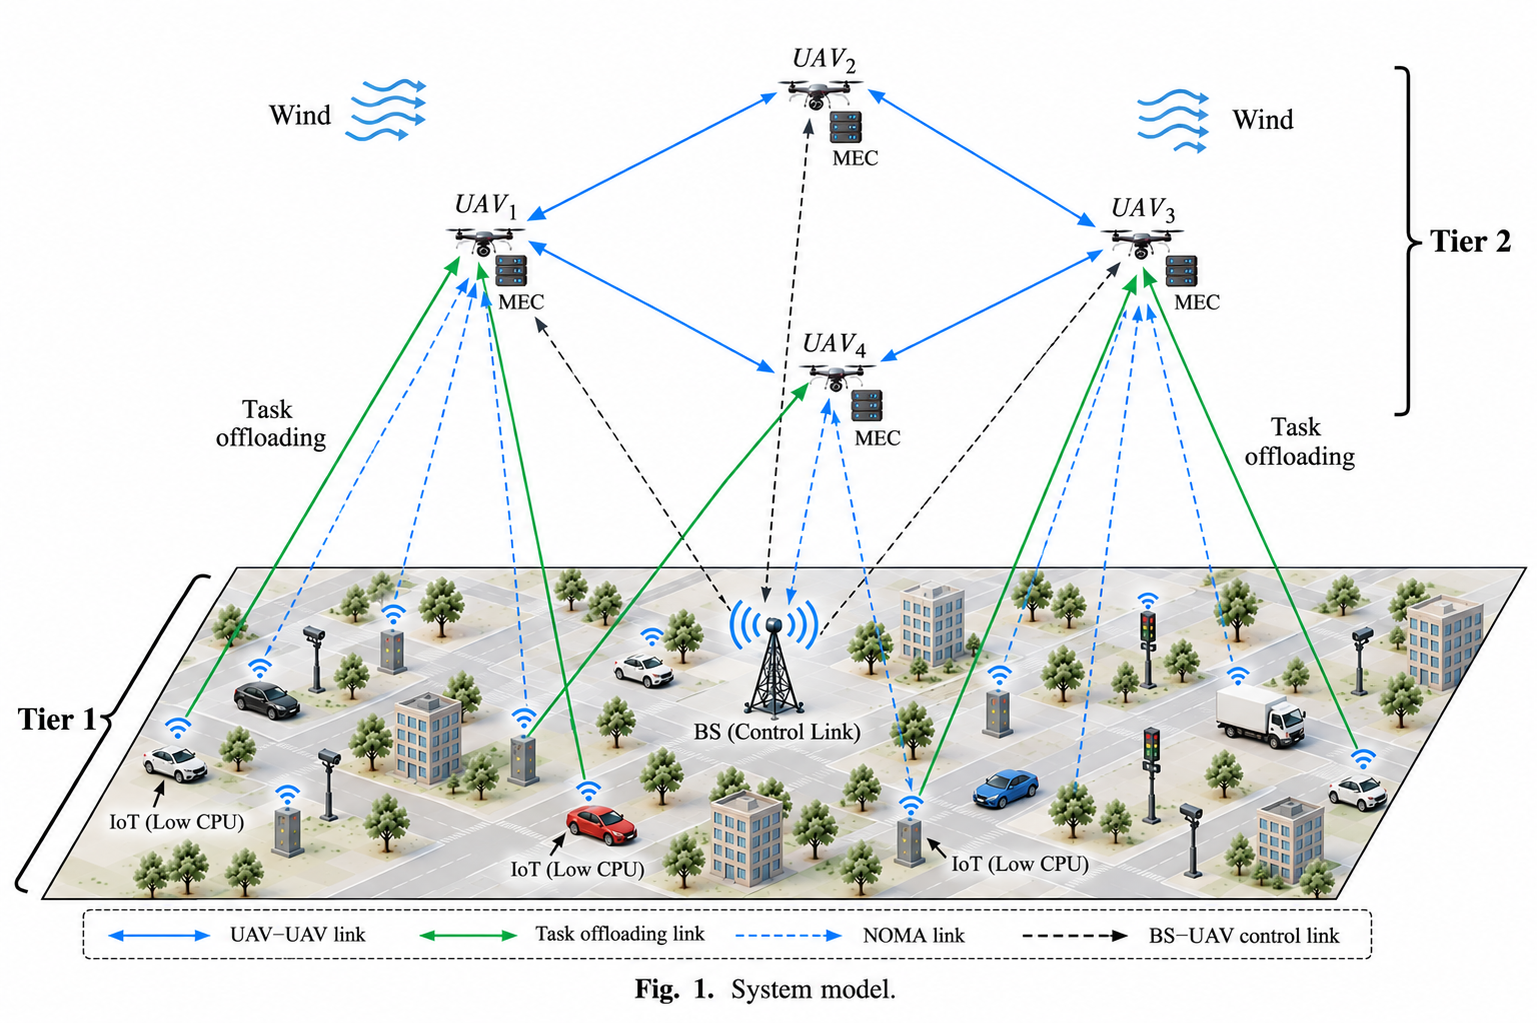
\includegraphics[width=\columnwidth]{figures/UAV-Assisted Edge Computing System Model.png}
  \caption{Architecture of the proposed priority-aware multi-UAV MEC-IoT network with NOMA-enabled uplink offloading, 3D aerial trajectories, and terrestrial coordination.}
  \label{fig:system_arch}
\end{figure}

\subsection{Network Architecture and Topology}

We consider an aerial-assisted mobile edge computing architecture serving a geographical operational domain $\mathcal{D} \subset \mathbb{R}^2$ over a finite operational horizon discretized into $T$ sequential time slots, indexed by $t \in \mathcal{T} \triangleq \{1, 2, \dots, T\}$, with uniform duration $\delta$. The network topology is depicted in Fig.~\ref{fig:system_arch} and comprises:
\begin{itemize}
    \item A set of terrestrial ground devices (GDs), indexed by $i \in \mathcal{I} \triangleq \{1, 2, \dots, I\}$, scattered across the service area. The horizontal coordinate of device $i$ at time slot $t$ is denoted by $\mathbf{u}_i[t] = [x_i[t], y_i[t], 0]^\top$. Each device possesses an internal computing processor characterized by maximum CPU clock frequency $f_i^{\mathrm{loc}}$.
    \item A fleet of rotary-wing UAVs, indexed by $j \in \mathcal{J} \triangleq \{1, 2, \dots, J\}$, functioning as flying MEC servers. Each UAV $j$ navigates in 3D airspace with instantaneous spatial coordinates
    \begin{equation}
    \mathbf{p}_j[t] = [x_j[t], y_j[t], z_j[t]]^\top, \quad z_j[t] \in [z_{\min}, z_{\max}],
    \end{equation}
    where $z_{\min}$ and $z_{\max}$ denote the allowable lower and upper operational altitude limits, respectively, mandated by obstacle clearance and aviation safety standards. Each UAV carries an onboard edge computing server operating at CPU clock frequency $f_j^{\mathrm{uav}}$.
    \item A terrestrial coordination station (Base Station, BS), located at fixed ground coordinates $\mathbf{w}_0 = [x_0, y_0, 0]^\top$, which serves as a central network synchronization anchor and offline training supervisor. The BS does not execute user computation tasks.
\end{itemize}

\subsection{3D UAV Kinematic and Fleet Mobility Model}

To provide responsive edge computing over the geographical region $\mathcal{D}$, each UAV $j \in \mathcal{J}$ navigates in three-dimensional airspace with time-varying coordinates $\mathbf{p}_j[t] = [x_j[t], y_j[t], z_j[t]]^\top \in \mathbb{R}^3$ at time slot $t \in \mathcal{T}$~\cite{li2026tnse}. The vertical movement of the aerial fleet is restricted within an authorized flight envelope $z_j[t] \in [z_{\min}, z_{\max}]$, where $z_{\min}$ and $z_{\max}$ denote the minimum safety clearance altitude and maximum regulatory ceiling, respectively. Furthermore, UAV horizontal flight is bounded by the operational domain, requiring $[x_j[t], y_j[t]]^\top \in \mathcal{D}$.

Following the continuous 3D aerial kinodynamic formulations in~\cite{li2026tnse} and~\cite{8937764}, the spatial displacement of UAV $j$ across consecutive time slots is governed by its instantaneous 3D velocity vector $\mathbf{v}_j[t] = [v_j^x[t], v_j^y[t], v_j^z[t]]^\top \in \mathbb{R}^3$. The discrete-time spatial kinematic evolution is modeled as
\begin{equation}
    \mathbf{p}_j[t+1] = \mathbf{p}_j[t] + \mathbf{v}_j[t] \delta, \quad \forall j \in \mathcal{J}, \; \forall t \in \mathcal{T},
    \label{eq:uav_pos_update}
\end{equation}
which decomposes along the Cartesian axes into
\begin{align}
    x_j[t+1] &= x_j[t] + v_j^x[t] \delta, \label{eq:uav_pos_x}\\
    y_j[t+1] &= y_j[t] + v_j^y[t] \delta, \label{eq:uav_pos_y}\\
    z_j[t+1] &= z_j[t] + v_j^z[t] \delta. \label{eq:uav_pos_z}
\end{align}
The instantaneous 3D flight speed is constrained by the aerodynamic performance limits of the rotorcraft:
\begin{equation}
    v_j[t] \triangleq \|\mathbf{v}_j[t]\|_2 = \sqrt{\bigl(v_j^x[t]\bigr)^2 + \bigl(v_j^y[t]\bigr)^2 + \bigl(v_j^z[t]\bigr)^2} \le V_{\max},
    \label{eq:uav_max_speed}
\end{equation}
where $V_{\max}$ is the maximum achievable flight speed. To prevent catastrophic mid-air collisions among aerial servers during cooperative fleet maneuvers, a minimum inter-UAV safety distance $d_{\min}$ must be maintained across all pairs of UAVs at every time slot:
\begin{equation}
    \|\mathbf{p}_j[t] - \mathbf{p}_{j'}[t]\|_2 \ge d_{\min}, \quad \forall j \neq j' \in \mathcal{J}, \; \forall t \in \mathcal{T}.
    \label{eq:collision_avoidance_dist}
\end{equation}

\subsection{Gauss-Markov Mobility Model of Ground Devices}

To capture realistic mobile IoT scenarios, GDs move autonomously within region $\mathcal{D}$. Following the Gauss-Markov (GM) random mobility formulation~\cite{11395508, li2026tnse}, temporal memory in device velocity and trajectory orientation is explicitly modeled. At each time slot $t \in \mathcal{T}$, the scalar velocity $v_i[t]$ and horizontal azimuth heading angle $\varphi_i[t]$ of device $i$ evolve recursively according to
\begin{align}
    v_i[t] &= \alpha_v v_i[t-1] + (1 - \alpha_v)\bar{v}_i + \sqrt{1 - \alpha_v^2}\,\zeta_i^v[t], \label{eq:gm_speed}\\
    \varphi_i[t] &= \alpha_\varphi \varphi_i[t-1] + (1 - \alpha_\varphi)\bar{\varphi}_i + \sqrt{1 - \alpha_\varphi^2}\,\zeta_i^\varphi[t], \label{eq:gm_direction}
\end{align}
where $\bar{v}_i$ and $\bar{\varphi}_i$ represent the asymptotic mean velocity and directional drift of device $i$, respectively. The coefficients $\alpha_v, \alpha_\varphi \in [0, 1]$ parameterize the correlation memory of the Markovian process, while $\zeta_i^v[t] \sim \mathcal{N}(0, \sigma_v^2)$ and $\zeta_i^\varphi[t] \sim \mathcal{N}(0, \sigma_\varphi^2)$ represent independent Gaussian stochastic driving noises. Consequently, the 2D position vector of device $i$ updates as
\begin{align}
    x_i[t] &= x_i[t-1] + \delta \cdot v_i[t-1] \cos\varphi_i[t-1], \label{eq:pos_x}\\
    y_i[t] &= y_i[t-1] + \delta \cdot v_i[t-1] \sin\varphi_i[t-1]. \label{eq:pos_y}
\end{align}
Should an updated coordinate fall outside the boundary of $\mathcal{D}$, a specular reflection boundary condition is applied to reverse its normal heading component, maintaining all ground nodes within the designated surveillance zone.

\subsection{Air-to-Ground Probabilistic Channel Model}

The wireless links connecting ground devices to aerial UAVs are governed by elevation-dependent probabilistic air-to-ground (A2G) propagation models~\cite{11500527, li2026tnse}. For device $i \in \mathcal{I}$ and UAV $j \in \mathcal{J}$ at slot $t$, the 3D Euclidean distance is
\begin{equation}
\begin{split}
    d_{i,j}[t] &= \|\mathbf{p}_j[t] - \mathbf{u}_i[t]\|_2 \\
    &= \sqrt{\bigl(x_j[t] - x_i[t]\bigr)^2 + \bigl(y_j[t] - y_i[t]\bigr)^2 + z_j^2[t]},
\end{split}
\label{eq:dist_wd_uav}
\end{equation}
and the corresponding spatial elevation angle (in degrees) is given by
\begin{equation}
    \psi_{i,j}[t] = \frac{180}{\pi} \arcsin\!\left(\frac{z_j[t]}{d_{i,j}[t]}\right).
    \label{eq:elev_angle}
\end{equation}
The probability of establishing a line-of-sight (LoS) link depends on the elevation angle and the propagation environment:
\begin{equation}
    \mathbb{P}^{\mathrm{LoS}}_{i,j}[t] = \frac{1}{1 + c_1 \exp\!\left(-c_2\bigl(\psi_{i,j}[t] - c_1\bigr)\right)},
    \label{eq:los_prob}
\end{equation}
where $c_1$ and $c_2$ denote environment-specific empirical parameters (e.g., urban, suburban, dense urban). The complementary non-line-of-sight (NLoS) probability is
\begin{equation}
    \mathbb{P}^{\mathrm{NLoS}}_{i,j}[t] = 1 - \mathbb{P}^{\mathrm{LoS}}_{i,j}[t].
\end{equation}
Let $\varrho_{\mathrm{LoS}}$ and $\varrho_{\mathrm{NLoS}}$ denote the large-scale channel attenuation coefficients for LoS and NLoS states, respectively, satisfying $\varrho_{\mathrm{LoS}} > \varrho_{\mathrm{NLoS}} > 0$. Accounting for geometric spreading with path-loss exponent $\alpha_{\mathrm{pl}}$, the effective A2G channel power gain is expressed as
\begin{equation}
\begin{split}
    h_{i,j}[t] &= \mathbb{P}^{\mathrm{LoS}}_{i,j}[t]\, h_{i,j}^{\mathrm{LoS}}[t] + \mathbb{P}^{\mathrm{NLoS}}_{i,j}[t]\, h_{i,j}^{\mathrm{NLoS}}[t] \\
    &= \Bigl[\mathbb{P}^{\mathrm{LoS}}_{i,j}[t] \varrho_{\mathrm{LoS}} + \mathbb{P}^{\mathrm{NLoS}}_{i,j}[t] \varrho_{\mathrm{NLoS}}\Bigr] \bigl(d_{i,j}[t]\bigr)^{-\alpha_{\mathrm{pl}}}.
\end{split}
\label{eq:channel_gain_a2g}
\end{equation}

\subsection{NOMA-Enhanced Uplink Transmission Model}

To enable multiple GDs to simultaneously offload workloads to a shared aerial server over identical bandwidth, power-domain non-orthogonal multiple access (NOMA) is employed on the uplink~\cite{11020655}. Let binary decision variable $\chi_{i,j}[t] \in \{0, 1\}$ indicate the device-UAV association, where $\chi_{i,j}[t] = 1$ denotes that device $i$ offloads its computation packet to UAV $j$ during slot $t$, and $\chi_{i,j}[t] = 0$ otherwise. Each GD may associate with at most one UAV per time slot:
\begin{equation}
    \sum_{j \in \mathcal{J}} \chi_{i,j}[t] \le 1, \quad \forall i \in \mathcal{I}, \; \forall t \in \mathcal{T}.
    \label{eq:assoc_constraint}
\end{equation}
Let $\mathcal{S}_j[t] \triangleq \{i \in \mathcal{I} : \chi_{i,j}[t] = 1\}$ denote the NOMA multiplexing cluster served by UAV $j$ at time slot $t$. To preserve receiver processing feasibility and prevent prohibitive successive interference cancellation (SIC) decoding delays, the multiplexing cluster size is bounded by
\begin{equation}
    |\mathcal{S}_j[t]| \le S_{\max}, \quad \forall j \in \mathcal{J}, \; \forall t \in \mathcal{T}.
    \label{eq:noma_cluster_limit}
\end{equation}
Let $p_i[t]$ denote the uplink transmission power assigned to device $i$ at slot $t$, constrained by physical amplifier limits $0 \le p_i[t] \le P_i^{\max}$. At the receiver of UAV $j$, SIC is applied to decode superimposed signals. Signals are decoded in ascending order of effective channel gains~\cite{11020655}. Let $\varpi_j[t]$ represent the permutation over $\mathcal{S}_j[t]$ satisfying
\begin{equation}
    h_{\varpi_j^{(1)}[t], j}[t] \le h_{\varpi_j^{(2)}[t], j}[t] \le \dots \le h_{\varpi_j^{(|\mathcal{S}_j[t]|)}[t], j}[t].
\end{equation}
Under ideal SIC, the signal of device $i = \varpi_j^{(r)}[t]$ experiences interference only from signals of devices with stronger channel gains (stages $r+1, \dots, |\mathcal{S}_j[t]|$). The received signal-to-interference-plus-noise ratio (SINR) is given by
\begin{equation}
    \Gamma_{i,j}[t] = \frac{p_i[t] h_{i,j}[t]}{\sum_{l = r+1}^{|\mathcal{S}_j[t]|} p_{\varpi_j^{(l)}[t]}[t] h_{\varpi_j^{(l)}[t], j}[t] + \sigma_n^2},
    \label{eq:sinr_noma}
\end{equation}
where $\sigma_n^2$ denotes the additive white Gaussian noise (AWGN) power at the UAV antenna. Given system bandwidth $W$ allocated to the cluster, the achievable uplink transmission data rate is
\begin{equation}
    R_{i,j}[t] = \chi_{i,j}[t] \, W \log_2\!\bigl(1 + \Gamma_{i,j}[t]\bigr).
    \label{eq:rate_noma}
\end{equation}
To ensure minimum transmission reliability, the achievable rate must satisfy the quality-of-service (QoS) threshold:
\begin{equation}
    R_{i,j}[t] \ge \chi_{i,j}[t] \, R_i^{\mathrm{th}}, \quad \forall i, j, t.
    \label{eq:qos_constraint}
\end{equation}

\subsection{Multi-Class Task Arrival and Composite Priority Model}
\label{sec:task_priority}

\subsubsection{Stochastic Task Arrival}
At each time slot $t \in \mathcal{T}$, device $i \in \mathcal{I}$ generates a computation task with probability $p_{\mathrm{arr}}$. Let $\alpha_i[t] \in \{0, 1\}$ denote the binary task arrival indicator. An incoming task is characterized by the descriptor tuple
\begin{equation}
    \Phi_i[t] = \bigl(D_i[t], \, C_i[t], \, \tau_i^{\max}[t], \, \kappa_i[t]\bigr),
    \label{eq:task_tuple}
\end{equation}
where $D_i[t]$ represents the raw input data payload (in bits), $C_i[t]$ denotes the required processing workload (in CPU execution cycles), $\tau_i^{\max}[t]$ specifies the delay deadline (in seconds), and $\kappa_i[t] \in \mathcal{K}_{\mathrm{app}}$ indicates the application category (e.g., safety-critical alarms, video analytics, environmental sensing).

\subsubsection{Composite Priority Formulation}
To differentiate heterogeneous workloads, we introduce a composite priority score $\Omega_i[t]$ for each active task:
\begin{equation}
    \Omega_i[t] = \mu_u \cdot \Omega_i^{\mathrm{urg}}[t] + \mu_c \cdot \Omega_i^{\mathrm{cls}}[t],
    \label{eq:priority_weight}
\end{equation}
where $\mu_u, \mu_c \ge 0$ are weighting parameters satisfying $\mu_u + \mu_c = 1$, governing the relative emphasis between deadline urgency and application criticality.

\textbf{Urgency Metric ($\Omega_i^{\mathrm{urg}}$):} The urgency term is modeled as an inverse linear mapping of the task deadline relative to system-wide bounds:
\begin{equation}
    \Omega_i^{\mathrm{urg}}[t] = \frac{\tau_{\max} - \tau_i^{\max}[t]}{\tau_{\max} - \tau_{\min} + \epsilon_0},
    \label{eq:urgency}
\end{equation}
where $\tau_{\max}$ and $\tau_{\min}$ are the maximum and minimum task deadlines in the network, respectively, and $\epsilon_0 > 0$ prevents division by zero. Tasks with shorter deadlines receive higher urgency values.

\textbf{Application Criticality Metric ($\Omega_i^{\mathrm{cls}}$):} Workload importance is assigned based on application type:
\begin{equation}
    \Omega_i^{\mathrm{cls}}[t] = w_{\kappa_i[t]},
    \label{eq:type_weight}
\end{equation}
where $w_\kappa \in (0, 1]$ denotes the predefined importance coefficient for class $\kappa \in \mathcal{K}_{\mathrm{app}}$. Critical events (e.g., collision avoidance, fire detection) are assigned higher weights than routine telemetry. Fig.~\ref{fig:priority_model} depicts the composite priority evaluation workflow.

\begin{figure}[!ht]
  \centering
  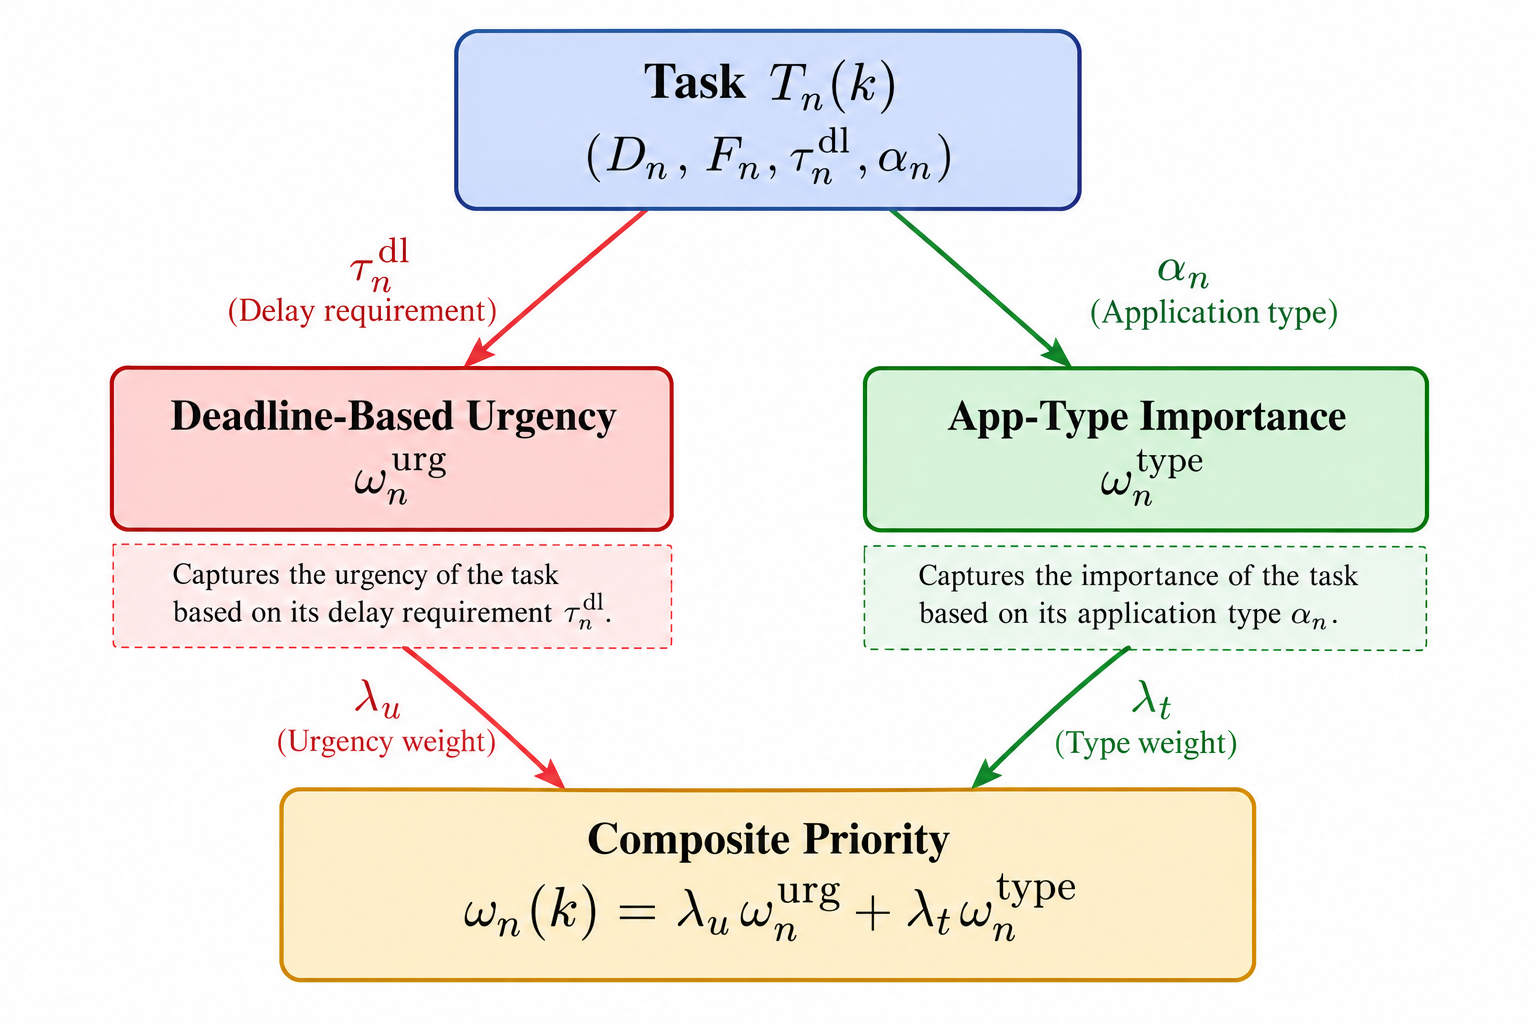
\includegraphics[width=0.95\columnwidth]{figures/Task Priority Computation Flowchart.png}
  \caption{Flowchart of the composite task priority evaluation integrating deadline urgency and application criticality.}
  \label{fig:priority_model}
\end{figure}

\subsection{Computation Latency and Queueing Dynamics}
\label{sec:computation_model}

\subsubsection{Execution Mode Selection}
Each generated task $\Phi_i[t]$ is processed either locally at the originating GD or offloaded to one serving UAV. Let $\chi_i^{\mathrm{loc}}[t] \in \{0, 1\}$ denote the local execution decision. The task assignment constraint enforces
\begin{equation}
    \chi_i^{\mathrm{loc}}[t] + \sum_{j \in \mathcal{J}} \chi_{i,j}[t] = \alpha_i[t], \quad \forall i \in \mathcal{I}, \; \forall t \in \mathcal{T}.
    \label{eq:exec_assign}
\end{equation}

\subsubsection{Local Computation Latency}
When $\chi_i^{\mathrm{loc}}[t] = 1$, task $\Phi_i[t]$ is processed on device $i$ at clock frequency $f_i^{\mathrm{loc}}$, incurring a local execution delay of
\begin{equation}
    T_i^{\mathrm{loc}}[t] = \frac{C_i[t]}{f_i^{\mathrm{loc}}}, \quad \forall i \in \mathcal{I}, \; \forall t \in \mathcal{T}.
    \label{eq:local_delay}
\end{equation}

\subsubsection{UAV Remote Offloading Latency}
When $\chi_{i,j}[t] = 1$, task $\Phi_i[t]$ is transmitted to UAV $j$. The end-to-end offloading latency consists of uplink transmission, queue buffering, and edge execution delays. The transmission delay over the wireless link is
\begin{equation}
    T_{i,j}^{\mathrm{tx}}[t] = \frac{D_i[t]}{R_{i,j}[t]}.
    \label{eq:tx_delay}
\end{equation}
Each UAV $j$ manages a first-in-first-out (FIFO) computation queue. Let $Q_j[t]$ denote the backlog workload (in CPU cycles) buffered at UAV $j$ at the start of slot $t$. The queue backlog evolves as
\begin{equation}
    Q_j[t+1] = \max\Biggl\{Q_j[t] + \sum_{i \in \mathcal{I}} \chi_{i,j}[t] \alpha_i[t] C_i[t] - f_j^{\mathrm{uav}}\delta, \; 0\Biggr\}.
    \label{eq:queue_update}
\end{equation}
The queue waiting delay experienced by incoming tasks at slot $t$ is
\begin{equation}
    W_j[t] = \frac{Q_j[t]}{f_j^{\mathrm{uav}}}.
    \label{eq:queue_delay}
\end{equation}
Once scheduled on the edge processor, the execution delay on UAV $j$ is
\begin{equation}
    T_{i,j}^{\mathrm{cmp}}[t] = \frac{C_i[t]}{f_j^{\mathrm{uav}}}.
    \label{eq:uav_cmp_delay}
\end{equation}
Summing these components, the total remote execution latency at UAV $j$ is
\begin{equation}
    T_{i,j}^{\mathrm{uav}}[t] = T_{i,j}^{\mathrm{tx}}[t] + W_j[t] + T_{i,j}^{\mathrm{cmp}}[t].
    \label{eq:total_uav_delay}
\end{equation}

\subsubsection{Overall Priority-Weighted Network Latency}
The overall completion latency for device $i$ at slot $t$ is expressed as
\begin{equation}
    T_i^{\mathrm{task}}[t] = \chi_i^{\mathrm{loc}}[t] T_i^{\mathrm{loc}}[t] + \sum_{j \in \mathcal{J}} \chi_{i,j}[t] T_{i,j}^{\mathrm{uav}}[t].
    \label{eq:total_delay}
\end{equation}
To prioritize time-sensitive and safety-critical requests, we define the system-wide priority-weighted average latency over all generated tasks across the mission horizon as
\begin{equation}
    \bar{T}_{\mathrm{pri}} = \frac{\sum_{t \in \mathcal{T}} \sum_{i \in \mathcal{I}} \alpha_i[t]\, \Omega_i[t]\, T_i^{\mathrm{task}}[t]}{\sum_{t \in \mathcal{T}} \sum_{i \in \mathcal{I}} \alpha_i[t]\, \Omega_i[t]}.
    \label{eq:avg_delay_priority}
\end{equation}
Under this formulation, delays incurred by high-priority tasks are penalized more heavily, guiding the scheduling policy to prioritize critical workloads.

\subsection{Energy Consumption Model}
\label{sec:energy_model}

Network energy consumption comprises ground device computing, wireless offloading transmission, UAV edge computing, and aerodynamic UAV propulsion energy.

\subsubsection{Ground Device Energy Consumption}
Following the dynamic voltage and frequency scaling (DVFS) circuit model, the computing energy consumed locally by device $i$ across horizon $T$ is
\begin{equation}
    E_i^{\mathrm{loc}} = \sum_{t \in \mathcal{T}} \chi_i^{\mathrm{loc}}[t] \alpha_i[t] \, \xi_i^{\mathrm{dev}} \bigl(f_i^{\mathrm{loc}}\bigr)^2 C_i[t],
    \label{eq:wd_loc_energy_total}
\end{equation}
where $\xi_i^{\mathrm{dev}}$ denotes the switched capacitance coefficient of the device processor. The wireless transmission energy expended during task offloading is
\begin{equation}
    E_i^{\mathrm{tx}} = \sum_{t \in \mathcal{T}} \sum_{j \in \mathcal{J}} \chi_{i,j}[t] \alpha_i[t] \, \frac{p_i[t] D_i[t]}{R_{i,j}[t]}.
    \label{eq:wd_tx_energy_total}
\end{equation}

\subsubsection{UAV Energy Consumption}
For each aerial server $j$, energy consumption includes onboard computation and aerodynamic propulsion:
\begin{equation}
    E_j^{\mathrm{total}} = E_j^{\mathrm{cmp}} + E_j^{\mathrm{fly}}.
    \label{eq:uav_energy_components}
\end{equation}
The server computation energy is given by
\begin{equation}
    E_j^{\mathrm{cmp}} = \sum_{t \in \mathcal{T}} \sum_{i \in \mathcal{I}} \chi_{i,j}[t] \alpha_i[t] \, \xi_j^{\mathrm{uav}} \bigl(f_j^{\mathrm{uav}}\bigr)^2 C_i[t],
    \label{eq:uav_cmp_energy_total}
\end{equation}
where $\xi_j^{\mathrm{uav}}$ denotes the effective hardware capacitance of the UAV server.

For rotary-wing UAVs, aerodynamic propulsion power dominates battery depletion. Following the analytical rotary-wing power model established in~\cite{8937764} and adopted in~\cite{li2026tnse}, the propulsion power required by UAV $j$ traveling at instantaneous horizontal speed $v_j[t] = \frac{\|\mathbf{p}_j[t+1] - \mathbf{p}_j[t]\|_2}{\delta}$ is modeled as
\begin{equation}
\begin{split}
    P_j^{\mathrm{prop}}[t] &= P_0 \left(1 + \frac{3 v_j^2[t]}{U_{\mathrm{tip}}^2}\right) \\
    &\quad + P_i \left(\sqrt{1 + \frac{v_j^4[t]}{4 v_0^4}} - \frac{v_j^2[t]}{2 v_0^2}\right)^{\frac{1}{2}} \\
    &\quad + \frac{1}{2} d_0 \rho_{\mathrm{air}} s_{\mathrm{rotor}} A_{\mathrm{rotor}} v_j^3[t],
    \label{eq:uav_prop_power}
\end{split}
\end{equation}
where $P_0$ is the blade profile power in hovering state, $U_{\mathrm{tip}}$ denotes the rotor blade tip velocity, $P_i$ denotes the hover induced power, $v_0$ is the mean rotor induced speed during hover, $d_0$ is the aerodynamic fuselage drag coefficient, $\rho_{\mathrm{air}}$ is air density, $s_{\mathrm{rotor}}$ is the rotor solidity ratio, and $A_{\mathrm{rotor}}$ denotes the rotor disc actuator area. The total propulsion energy expended over the mission horizon is
\begin{equation}
    E_j^{\mathrm{fly}} = \delta \sum_{t = 1}^{T-1} P_j^{\mathrm{prop}}[t].
    \label{eq:uav_fly_energy_total}
\end{equation}
Each UAV must operate within its onboard battery capacity:
\begin{equation}
    E_j^{\mathrm{cmp}} + E_j^{\mathrm{fly}} \le E_j^{\max}, \quad \forall j \in \mathcal{J}.
    \label{eq:uav_energy_budget}
\end{equation}

\subsection{Joint Problem Formulation}

Our objective is to minimize the priority-weighted average task execution latency while penalizing UAV energy consumption, by jointly optimizing 3D UAV trajectories, priority-aware computation offloading assignments, and NOMA uplink transmit powers. We formulate this optimization problem as a stochastic MINLP:
\begin{equation}
\begin{aligned}
\min_{\mathcal{X}} \;\;
& \frac{\sum_{t \in \mathcal{T}} \sum_{i \in \mathcal{I}} \alpha_i[t] \, \Omega_i[t] \, T_i^{\mathrm{task}}[t]}{\sum_{t \in \mathcal{T}} \sum_{i \in \mathcal{I}} \alpha_i[t] \, \Omega_i[t]} \\
& + \lambda_{\mathrm{eng}} \sum_{t \in \mathcal{T}} \sum_{j \in \mathcal{J}} \left(E_j^{\mathrm{cmp}}[t] + \delta P_j^{\mathrm{prop}}[t]\right)
\end{aligned}
\label{eq:problem_obj}
\end{equation}
where $\lambda_{\mathrm{eng}} \ge 0$ is a regularization coefficient balancing latency minimization and energy conservation, and $\mathcal{X} = \{\mathbf{p}_j[t], \chi_{i,j}[t], \chi_i^{\mathrm{loc}}[t], p_i[t]\}_{\forall i, j, t}$ is the set of decision variables.

The optimization is subject to the following constraints:
\begin{align}
&\mathcal{C}_1:\; \chi_i^{\mathrm{loc}}[t] + \sum_{j \in \mathcal{J}} \chi_{i,j}[t] = \alpha_i[t], && \forall i \in \mathcal{I}, \, \forall t \in \mathcal{T}, \label{eq:c1}\\
&\mathcal{C}_2:\; 0 \le p_i[t] \le P_i^{\max}, && \forall i \in \mathcal{I}, \, \forall t \in \mathcal{T}, \label{eq:c2}\\
&\mathcal{C}_3:\; \|\mathbf{p}_j[t+1] - \mathbf{p}_j[t]\|_2 \le V_{\max} \delta, && \forall j \in \mathcal{J}, \, \forall t \in \mathcal{T}, \label{eq:c3}\\
&\mathcal{C}_4:\; z_{\min} \le z_j[t] \le z_{\max}, && \forall j \in \mathcal{J}, \, \forall t \in \mathcal{T}, \label{eq:c4}\\
&\mathcal{C}_5:\; \|\mathbf{p}_j[t] - \mathbf{p}_{j'}[t]\|_2 \ge d_{\min}, && \forall j \neq j' \in \mathcal{J}, \, \forall t \in \mathcal{T}, \label{eq:c5}\\
&\mathcal{C}_6:\; E_j^{\mathrm{cmp}} + E_j^{\mathrm{fly}} \le E_j^{\max}, && \forall j \in \mathcal{J}, \label{eq:c6}\\
&\mathcal{C}_7:\; [x_j[t], y_j[t]]^\top \in \mathcal{D}, && \forall j \in \mathcal{J}, \, \forall t \in \mathcal{T}, \label{eq:c7}\\
&\mathcal{C}_8:\; |\mathcal{S}_j[t]| \le S_{\max}, && \forall j \in \mathcal{J}, \, \forall t \in \mathcal{T}, \label{eq:c8}\\
&\mathcal{C}_9:\; R_{i,j}[t] \ge \chi_{i,j}[t] R_i^{\mathrm{th}}, && \forall i \in \mathcal{I}, \, j \in \mathcal{J}, \, t \in \mathcal{T}, \label{eq:c9}\\
&\mathcal{C}_{10}:\; T_i^{\mathrm{task}}[t] \le \tau_i^{\max}[t], && \forall i \in \mathcal{I}, \, \forall t \in \mathcal{T}. \label{eq:c10}
\end{align}

Constraint $\mathcal{C}_1$ guarantees mutually exclusive execution mode selection. Constraint $\mathcal{C}_2$ restricts device transmit power. Constraints $\mathcal{C}_3$--$\mathcal{C}_4$ enforce the UAV maximum airspeed and vertical altitude limits, respectively. Constraint $\mathcal{C}_5$ mandates the minimum inter-UAV spatial separation to eliminate mid-air collision risks. Constraints $\mathcal{C}_6$--$\mathcal{C}_7$ bound UAV battery budgets and operational territory borders. Constraint $\mathcal{C}_8$ limits the maximum NOMA cluster size to regulate SIC decoding complexity. Constraint $\mathcal{C}_9$ guarantees uplink data rates satisfy the minimum QoS threshold. Finally, constraint $\mathcal{C}_{10}$ enforces individual task latency deadlines.

\textit{Complexity and Tractability Remark:} Problem~\eqref{eq:problem_obj}--\eqref{eq:c10} is a stochastic MINLP characterized by binary assignment choices ($\chi_i^{\mathrm{loc}}, \chi_{i,j}$), continuous flight and power variables ($\mathbf{p}_j, p_i$), non-convex logarithmic rate expressions, non-linear aerodynamic functions, and stochastic task arrivals and device mobility. The problem is NP-hard, making traditional convex optimization approaches computationally intractable in real time. This motivates a multi-agent reinforcement learning paradigm to coordinate multi-UAV navigation, scheduling, and power adaptation under partial observability.

%% ============================================================
%%  IV. PROPOSED METHODOLOGY
%% ============================================================
\section{Proposed Methodology}
\label{section_IV}

\subsection{Multi-Agent Markov Decision Process (MAMDP) Formulation}
\label{sec:mamdp}

\subsubsection{Global State Space (\texorpdfstring{$\mathcal{S}$}{S})}

\subsubsection{Local Observation Space (\texorpdfstring{$\mathcal{O}_j$}{O\_j})}

\subsubsection{Action Space (\texorpdfstring{$\mathcal{A}_j$}{A\_j})}

\subsubsection{Reward Function Design}

\subsection{Analytical NOMA Power Allocation via Bisection}
\label{sec:noma_power}

\subsection{MAPPO Architecture and Policy Optimization}
\label{sec:mappo_arch}

%% ============================================================
%%  V. SIMULATION RESULTS
%% ============================================================
\section{Simulation Results}
\label{section_V}

\subsection{Simulation Configuration and Parameters}
\label{sec:sim_config}

\subsection{Performance Benchmarks}
\label{sec:benchmarks}

\subsection{Convergence and Training Dynamics}
\label{sec:sim_convergence}

\subsection{Priority-Weighted Latency Analysis}
\label{sec:sim_latency}

\subsection{UAV Energy Consumption and 3D Trajectory Adaptation}
\label{sec:sim_energy}

%% ============================================================
%%  VI. CONCLUSION AND FUTURE WORK
%% ============================================================
\section{Conclusion and Future Work}
\label{con}

\bibliographystyle{IEEEtran}
\bibliography{ref}

\end{document}
